\PassOptionsToPackage{utf8}{inputenc}
\documentclass{bioinfo}

\usepackage{makecell}

\usepackage{floatrow}

\usepackage{comment}

\usepackage{siunitx}

% singlelinecheck=false puts subcaptions on the left
\usepackage[singlelinecheck=false]{subcaption}

\usepackage{amsthm}
\theoremstyle{definition}
\newtheorem{definition}{Definition}[section]
\newtheorem{theorem}{Theorem}[section]
\newtheorem{corollary}{Corollary}[theorem]
\newtheorem{lemma}[theorem]{Lemma}

\usepackage{amsfonts}
\usepackage{booktabs}

\usepackage{algorithm2e}
\usepackage[usenames,dvipsnames]{xcolor}
\SetAlgoLined
\SetKwProg{for}{For}{:}{end}
\SetKwProg{pgsgd}{PG-SGD}{:}{end}
\SetKwProg{each}{For each}{:}{end}
\usepackage{bm}

% we squeeze our figures even more together
\captionsetup{belowskip=-2pt}

\SetAlgoLined
\SetKwProg{MyStruct}{Struct}{ contains}{end}

\newcommand{\vocab}{\textbf}
\newcommand{\red}[1]{{\textcolor{Red}{#1}}}
\newcommand{\FIXME}[1]{\red{[FIXME: #1]}}

\usepackage{orcidlink}
\hypersetup{hidelinks}


\def\labelitemi{--}

\copyrightyear{2023} \pubyear{XXXX}

\access{Advance Access Publication Date: Day Month Year}
\appnotes{Genome Analysis}

\begin{document}
\firstpage{1}

\subtitle{Genome Analysis}

\title[Pangenome graph layout by HOGWILD! Path-Guided Stochastic Gradient Descent]{Pangenome graph layout by HOGWILD! Path-Guided Stochastic Gradient Descent}
\author[Heumos, Guarracino \textit{et~al}.]{
Simon~Heumos\,$^{\orcidlink{0000-0003-3326-817X}1,2,\dagger,*}$,
Andrea~Guarracino\,$^{\orcidlink{0000-0001-9744-131X}3,4,\dagger}$,
Jan-Niklas Manuel Schmelzle\,$^{\orcidlink{0000-0001-8566-4049}5,6}$,
Jiajie Li\,$^{\orcidlink{0000-0002-9467-0659}6}$,
Zhiru Zhang\,$^{\orcidlink{0000-0002-0778-0308}6}$,
Sven Nahnsen\,$^{\orcidlink{0000-0002-4375-0691}1,2}$,
Pjotr Prins\,$^{\orcidlink{0000-0002-8021-9162}3}$,
Erik~Garrison\,$^{\orcidlink{0000-0003-3821-631X}\text{\sfb 3},*}$
}

\address{
$^1$Quantitative Biology Center (QBiC), University of Tübingen, Tübingen 72076, Germany \\
$^2$Biomedical Data Science, Department of Computer Science, University of Tübingen, Tübingen 72076, Germany \\
$^3$Department of Genetics, Genomics and Informatics, University of Tennessee Health Science Center, Memphis, TN 38163, USA \\
$^4$Genomics Research Centre, Human Technopole, Milan 20157, Italy \\
$^5$Department of Computer Engineering, School of Computation, Information and Technology (CIT), Technical University of Munich, Munich 80333, Germany \\
$^6$School of Electrical and Computer Engineering, Cornell University, Ithaca, NY 14853, USA \\
}

\corresp{
$^\ast$To whom correspondence should be addressed. \\
$^{\dagger}$The authors wish it to be known that, in their opinion, the first two authors should be regarded as Joint First Authors.\
}

\history{Received on XXXXX; revised on XXXXX; accepted on XXXXX}

\editor{Associate Editor: XXXXXXX}

\abstract{
\textbf{Motivation:}
The availability of many high-quality genomes has led to the need for models that allow the study of genetic variability within entire populations.
Pangenome graphs can represent the full diversity between multiple genomes, but they may exhibit complex structures due to common patterns of genome variation.
These nonlinear structures introduce difficulty in downstream analyses, visualization, and interpretation. \\
\textbf{Results:}
To address these challenges, we propose a novel layout algorithm, the Path-Guided Stochastic Gradient Descent (PG-SGD).
Our approach orders the nodes of a pangenome graph by leveraging the HOGWILD! strategy and it is guided by the path position information of the genomes represented in the graph.
We demonstrate that our implementation can efficiently compute the latent structure of gigabase-scale pangenome graphs, exposing their biological features. \\
\textbf{Availability:}
The PG-SGD algorithm is implemented in \textit{odgi} which is published as free software under the MIT open source license.
Source code is available at \url{https://github.com/pangenome/odgi} and documentation at \url{https://odgi.readthedocs.io/en/latest/rst/tutorials/sort_layout.html}.
\textit{odgi} can be installed via Bioconda \url{https://bioconda.github.io/recipes/odgi/README.html} or GNU Guix \url{https://github.com/ekg/guix-genomics/blob/master/odgi.scm}. \\
\textbf{Contact:} \href{simon.heumos@qbic.uni-tuebingen.de}{simon.heumos@qbic.uni-tuebingen.de},
\href{egarris5@uthsc.edu}{egarris5@uthsc.edu} \\
%\textbf{Supplementary information:} Supplementary data are available at \textit{Bioinformatics} online.
}

\maketitle


\section{Background}
A pangenome1 models the entire set of genomic elements of a given population. It can efficiently be encoded2 in the form of a variation graph, which embeds the linear sequences of the pangenome as paths in the graphs themselves. 
\\
In pangenome graphs models, DNA sequences are incorporated as nodes with edges connecting the nodes as they occur as sequences representing the graph.
\\
Pangenome graphs \cite{computational2016computational}. blubb.
\\
variation graph model
\\
SGD-layout. Layout in general.
\\ Very light background.
%Pangenome graphs built from raw sets of alignments may have complex structures generated by common patterns of genome variation.

\section{Algorithm}

\paragraph{The HOGHWILD! path-guided stochastic gradient descent algorithm}
Our algorithm is inspired by Zheng et al. (\url{https://doi.org/hkv4}) and it is theoretically applicable in any number of dimensions.
In this work, we describe the results in 1D and 2D.
In our implementation, the algorithm moves a single pair of nodes at a time, minimizing the disparity between the layout distance of a node pair and the actual nucleotide distance of a path traversing these nodes.
Our path index enables efficient navigation of path positions by updating nodes on the fly, instead of keeping all pairwise distances of all nodes in memory.
This allows the PG-SGD to be applied to gigabase-scale pangenome graphs. \\
Our multi-threaded implementation (\url{https://odgi.readthedocs.io/en/latest/rst/tutorials/sort_layout.html}) presents a working prototype that is based on succinct graph data structures (\url{https://doi.org/ghqdzw}):
\begin{itemize}
	\item The first node Xi of a pair is a uniform path step pick from all nodes.
	\item The second node Xj of a pair is sampled from the same path following a Zipfian distribution. 
	\item The path nucleotide distance of the nodes in the pair guides the actual layout distance dij update of these nodes. The magnitude r of the update depends on the current learning rate of the SGD.
\end{itemize}
%The exploration of the path-guided SGD parameter space is in progress, in order to get the best layout as quickly as possible.
We describe in algorithm~\ref{alg:pg_sgd} how the PG-SGD works on a single thread. We can have several worker threads but only one checker thread!

\begin{algorithm}
	\caption{Pseudocode of the PG-SGD algorithm. Explain $\eta$. Explain $PathIndex$ in the text. Explain $ZipfZetas$ in the text. Explain $RandomLayout$ in the text. Explain annealing schedule in the text or rephrase this wording.}
	\label{alg:pg_sgd}
	\pgsgd{\textbf{(}V\textbf{)}}{
		\textbf{input:} variation graph $V = (N, E, P)$ \\
		%https://tex.stackexchange.com/questions/22643/how-to-write-letters-in-bold-in-the-math-mode
		\textbf{output:} $k$-dimensional layout \boldsymbol{$L$} with $n$ nodes \\
		\boldsymbol{$P$} $\leftarrow PathIndex(G)$ \\ 
		\boldsymbol{$Z$} $\leftarrow ZipfZetas(G,P)$ \\ %@Andrea is this correct like this?
		\boldsymbol{$L$} $\leftarrow RandomLayout(n, k)$ \tcp{only 2D PG-SGD has a random layout initialization, 1D starts with the current node order}
		% atomic positions initialization?
		% TODO for somplicity reasons I would only describe the 2D one here
		\for{$\eta$ $in$ $annealing$ $schedule$}{
			\each{$term$ $update$} {
				random path step from all steps \\
				if cooling $||$ flip \\
				uniform step across the path \\
				else \\
				forward \\
				use Z to generate max jump length \\
				newsteprank = cursteprank + sampledzipfvalue \\
				backward \\
				use Z to generate jump length \\
				newsteprank = cursteprank + sampledzipfvalue \\
				get path positions via path index \\	
				$nuc\_dist=abs(pos\_in\_path\_a - pos\_in\_path\_b)$ \\
				$term\_weight = 1.0 / term\_dist$ \\
				$w\_ij = term\_weight$ \\
				$mu = eta.load() * w_{ij}$ \\
				$dx = X[i].load() - X[j].load()$ \tcp{calculate layout distance }
				$mag = std::abs(dx)$ \\
				$Delta = mu * (mag - d_ij) / 2$ \\
				$ Delta_abs = std::abs(Delta)$ \\
				\tcp{potentially store new Delta\_max}
				$r = Delta / mag$ \\
				$ r_x = r * dx$ \\
				\tcp{new X = old X - r\_x}
				\tcp{new Y = old Y - r\_Y, 2D only}
			}
		}
	}
\end{algorithm}

Fig. 1: Describe how our approach works, especially a single update operation (Fig. \ref{fig:sketches}). Explanation of 1D graph updating in Figures \ref{fig:1d_before_update}-\ref{fig:1d_after_update}. Explanation of 2D graph updating in Figures \ref{fig:2d_before_update}-\ref{fig:2d_after_update}. Zipfian distribution.

\begin{figure*}[!htb]
	\centering
		%\hline
		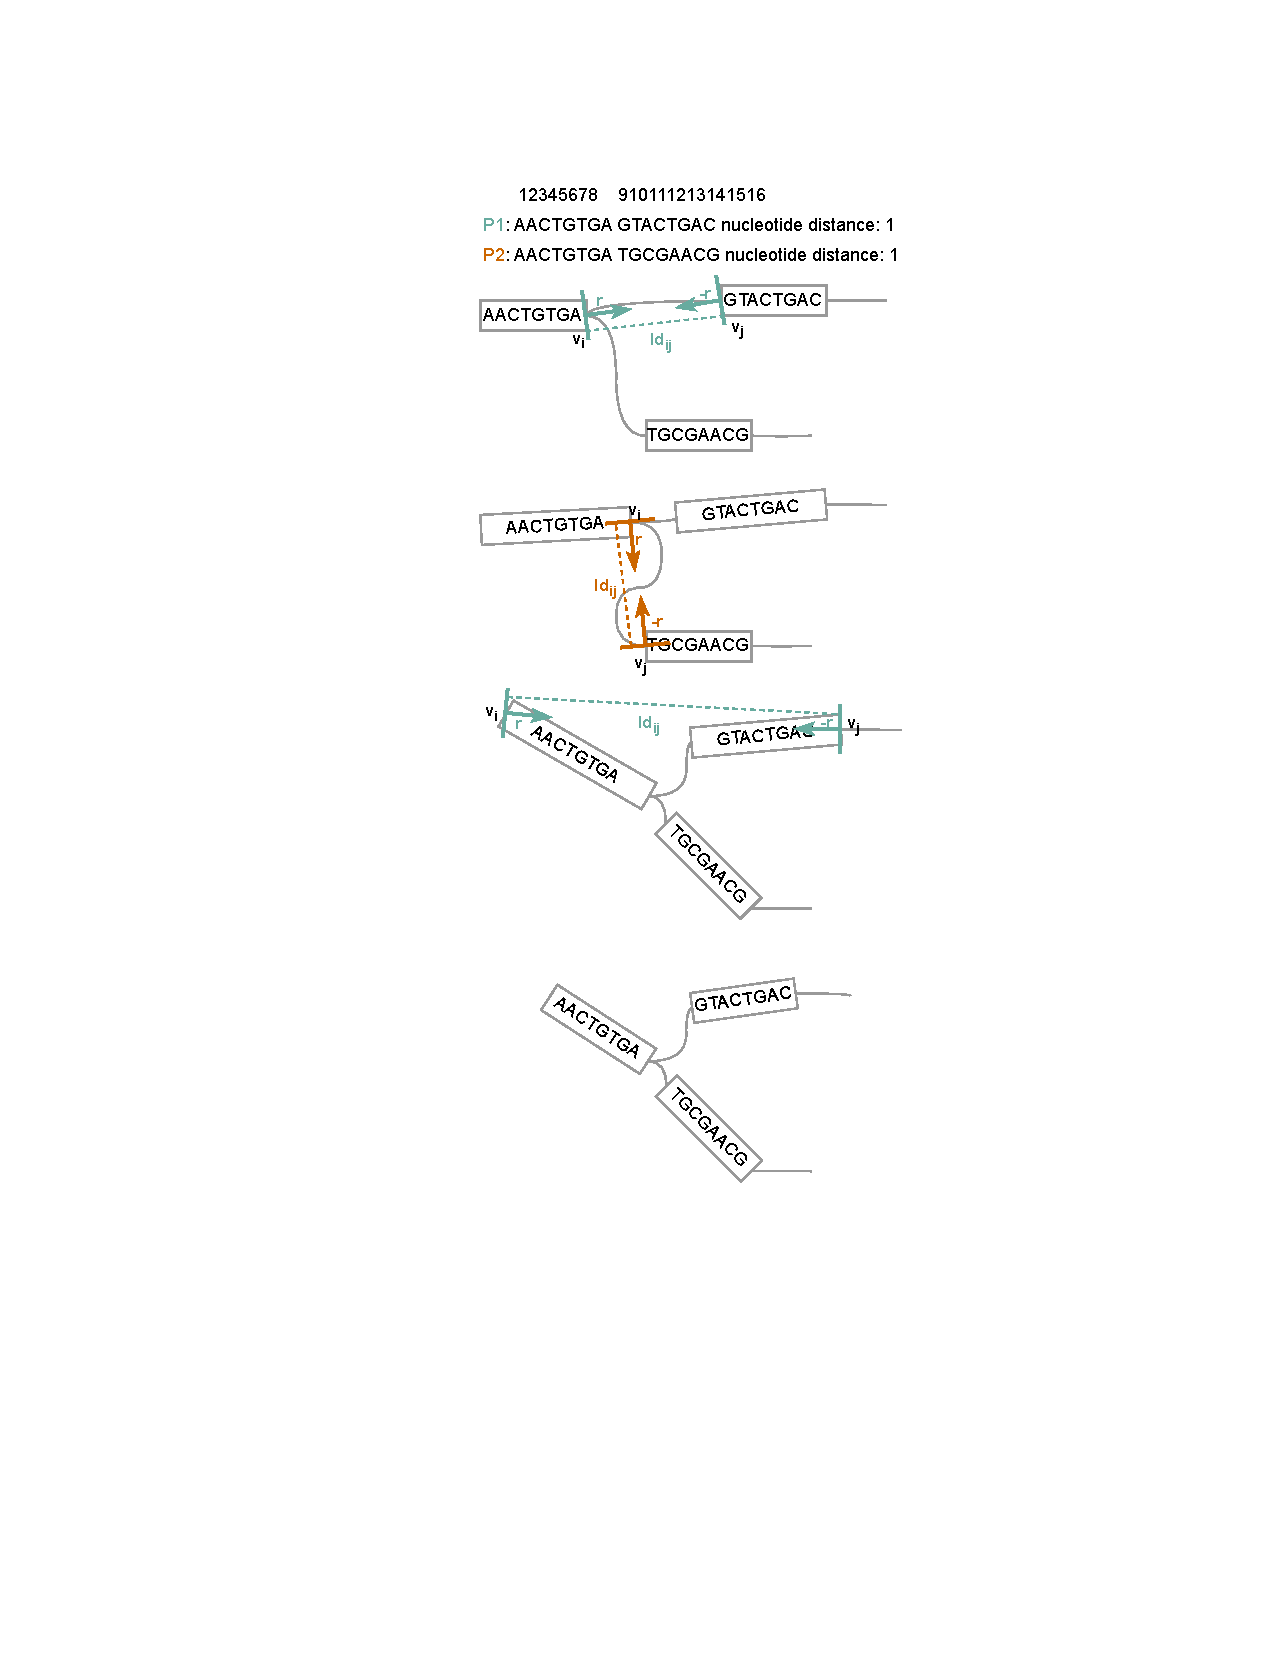
\includegraphics[width=\linewidth, trim=0cm 8cm 0cm 0cm, clip]{fig/sketches/PG-SGD.drawio.pdf}
	\caption{
		2D PG-SGD update operation sketches. \\
		\FIXME{ADD CAPTION.} \\ 
		\FIXME{PROVIDE SEVERAL NICE FIGURES SO WE CAN REARRANGE STUFF INTO SUBFIGURES.}
	}
	\label{fig:sketches}
\end{figure*}

\section{Results}
\label{sec:results}

%\subsection{Experimental insights}

%\subsection{Limitations}

% something for the supplementary
\paragraph{Performance evaluation}
Fig. 2: Performance evaluation 1D + 2D: Time + RAM by number of haplotypes (Fig.~\ref{fig:haps_time_ram}). Time + RAM by number of threads (Fig.~\ref{fig:threads_time_ram}). Full HPRC graph.
\\
1D (max. threads) vs. ALIBI; we should compare time + RAM in Fig.~\ref{fig:alibi}.
But also by our sorting goodness metrics: odgi sort + the one suggested in the ALIBI paper in Table 1.
\\
2D (max. threads) + odgi draw vs. Bandage in Fig.~\ref{fig:bandage}.
\begin{figure*}[!htb]
	\centering
	%\hline
	\begin{subfigure}[t]{0.4\textwidth}
		\centering
		\caption{}
		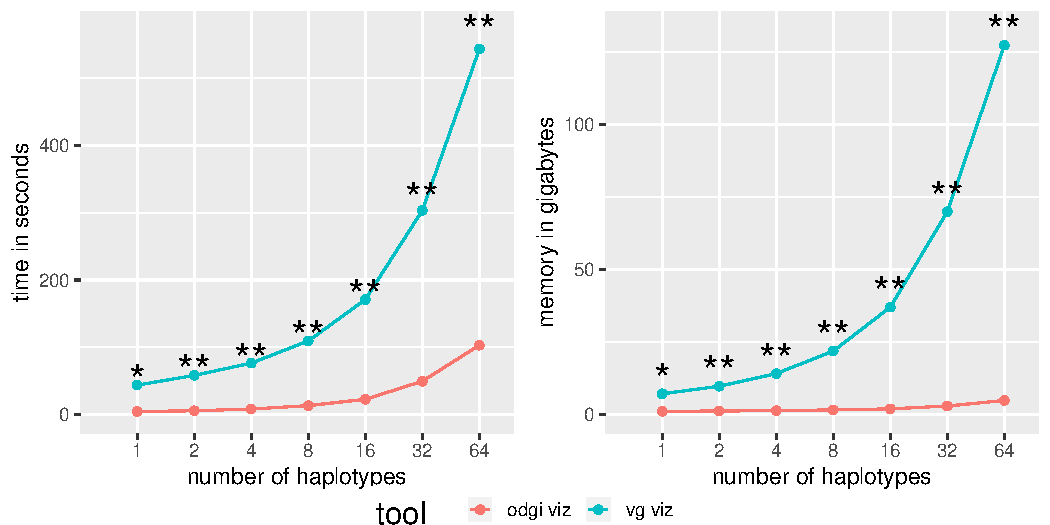
\includegraphics[width=\linewidth]{fig/performance/TODO_by_haps_eval_time_ram.pdf}
		\label{fig:haps_time_ram}
	\end{subfigure}
	\begin{subfigure}[t]{0.4\textwidth}
		\centering
		\caption{}
		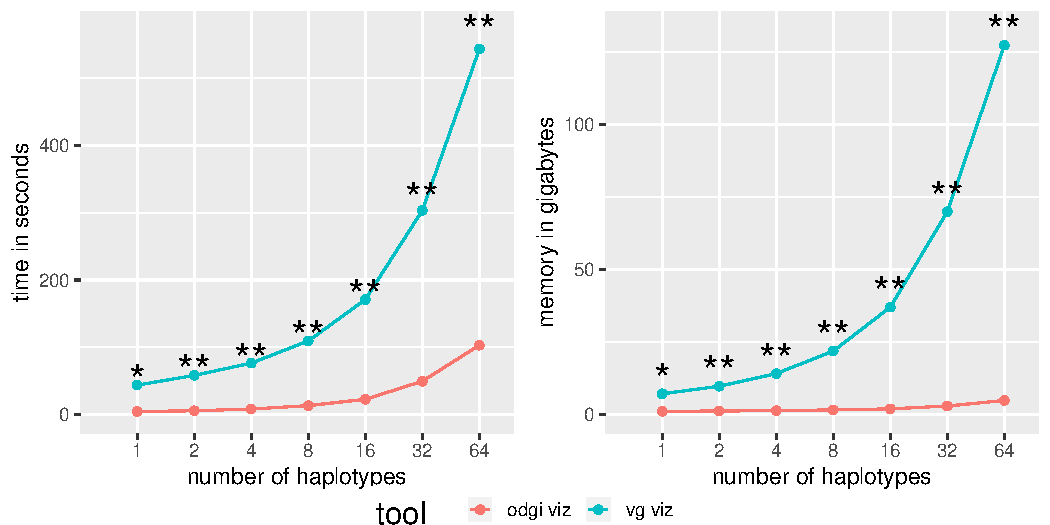
\includegraphics[width=\linewidth]{fig/performance/TODO_by_threads_eval_time_ram.pdf}
		\label{fig:threads_time_ram}
	\end{subfigure}
	%\smallskip
	\begin{subfigure}[t]{0.4\textwidth}
		\centering
		\caption{}
		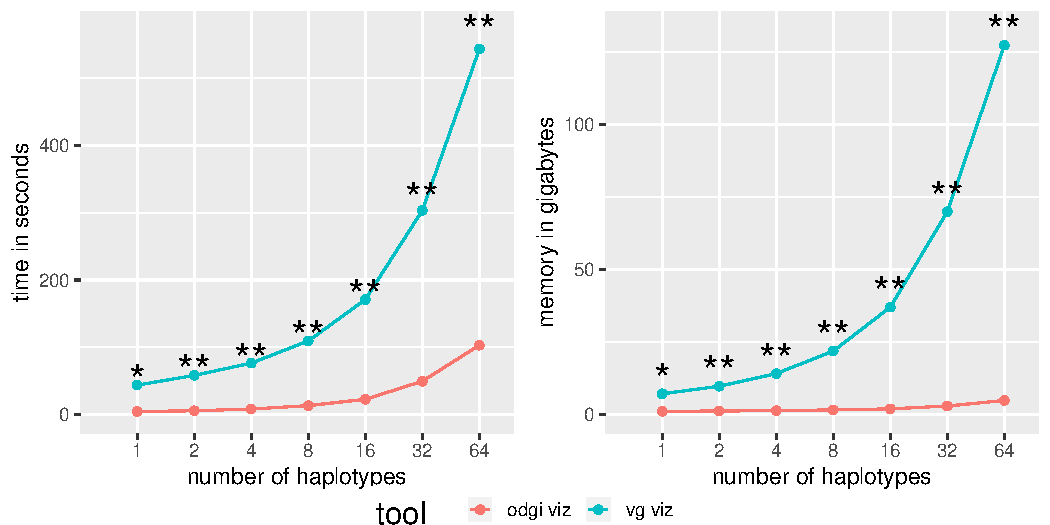
\includegraphics[width=\linewidth]{fig/performance/TODO_1d_alibi_time_ram.pdf}
		\label{fig:alibi}
	\end{subfigure}
	\begin{subfigure}[t]{0.4\textwidth}
		\centering
		\caption{}
		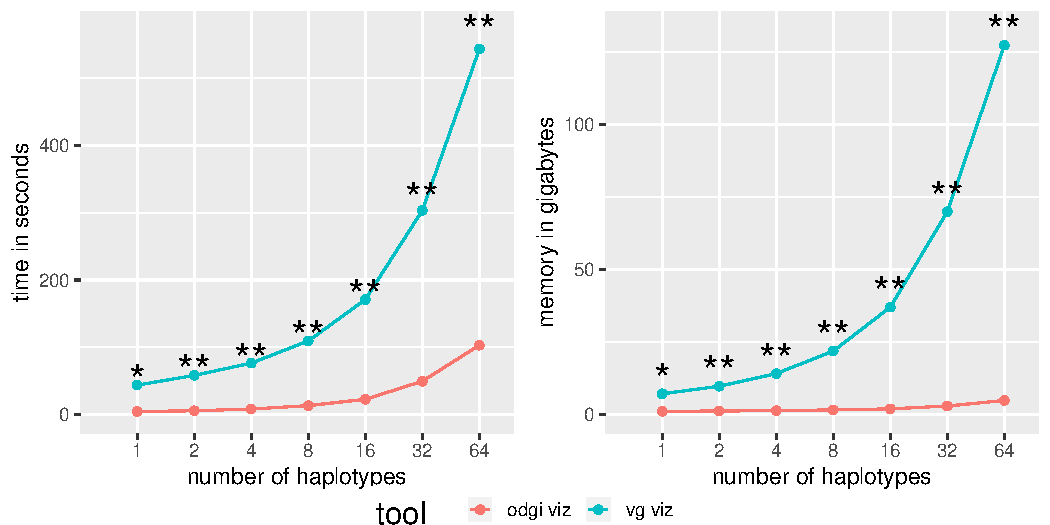
\includegraphics[width=\linewidth]{fig/performance/TODO_by_2d_draw_bandage_time_ram.pdf}
		\label{fig:bandage}
	\end{subfigure}
	\caption{
		Performance evaluations.
		\textbf{(a)} PG-SGD 1D and 2D by haplotypes. \textbf{(b)} PG-SGD 1D and 2D by threads. \textbf{(c)} PG-SGD vs. ALIBI. \textbf{(d)} PG-SGD + draw vs. BANDAGE.
	}
	\label{fig:performance}
\end{figure*}
\\
\\
Table 1: Metrics of the ALIBI and PG-SGD graphs from Fig. 2.
\begin{table}[]
	\caption{Metrics of the 1D PG-SGD and ALIBI graphs.}
	\begin{tabular}{|l|l|l|}
		\hline
		& 1D PG-SGD & ALIBI \\ \hline
		METRIC 1 &           &       \\ \hline
		METRIC 2 &           &       \\ \hline
	\end{tabular}
\end{table}
Already, the PG-SGD outperforms existing graph linearization methods like the flow procedure (\url{https://doi.org/gdw58w}) or ALIBI (\url{https://doi.org/hkv3}).
\paragraph{Latent graph structure reveals underlying biology}
Fig. 3: Cool quantitative 1D sortings and 2D layouts: biological implications.
Randomly sorted. PG-SGD sorted. Ygs sorted. Reference sorted.
We want a pipeline of sortings. 2D layout of the whole HPRC.
Chr6 HPRC HLA graph? Chr8 beta-defensin gene cluster HPRC? Whole HPRC?
\\
We could also try to build a gastric cancer pangenome graph with data from \url{https://www.nature.com/articles/s41467-022-33073-7} from up to 185 samples.
However, we would have to request access to the data.
\\
\\
\begin{figure*}[!htb]
	\centering
	%\hline
	\begin{subfigure}[t]{0.4\textwidth}
		\centering
		\caption{}
		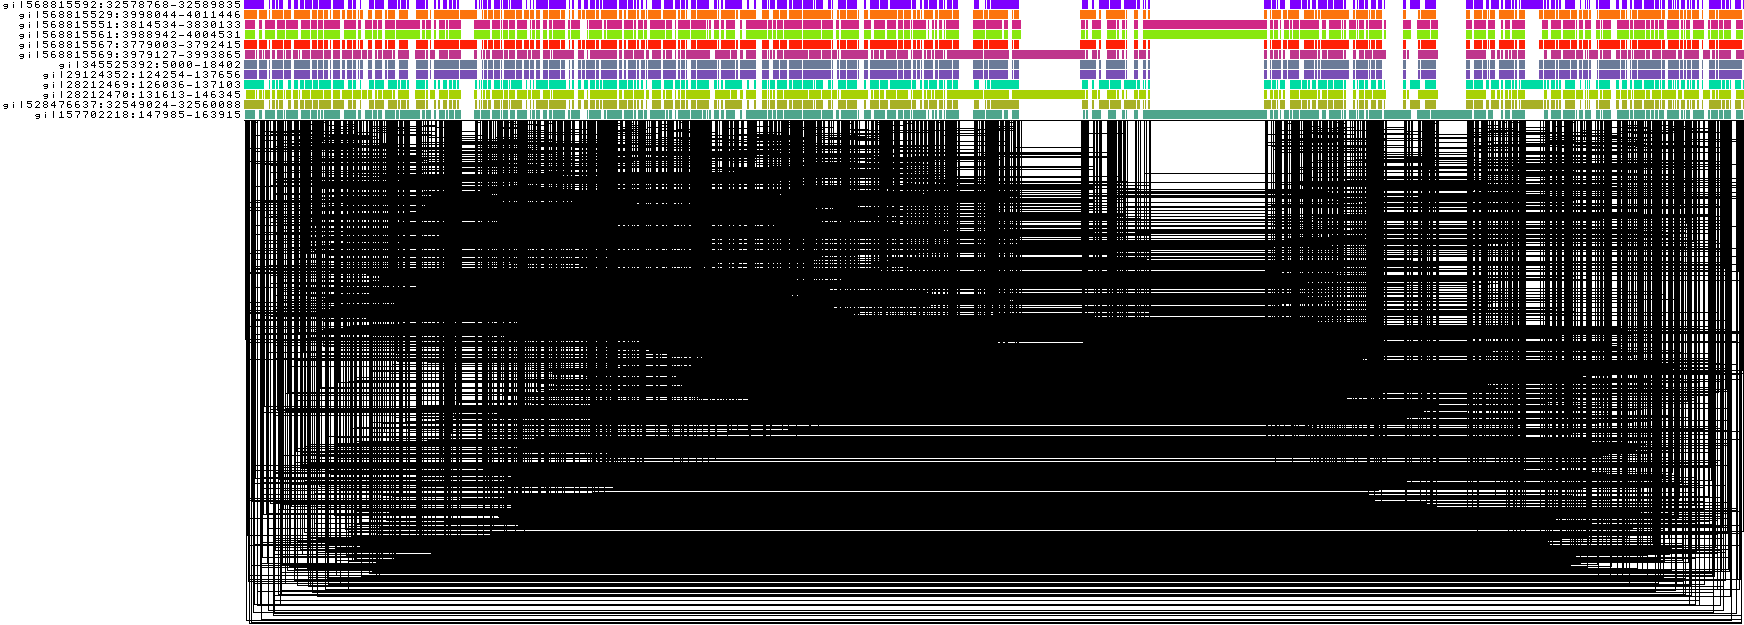
\includegraphics[width=\linewidth]{fig/latent_graph_structure/DRB1-3123.fa.gz.c666522.417fcdf.seqwish.og.r.og.png}
		\label{fig:random}
	\end{subfigure}
	\begin{subfigure}[t]{0.4\textwidth}
		\centering
		\caption{}
		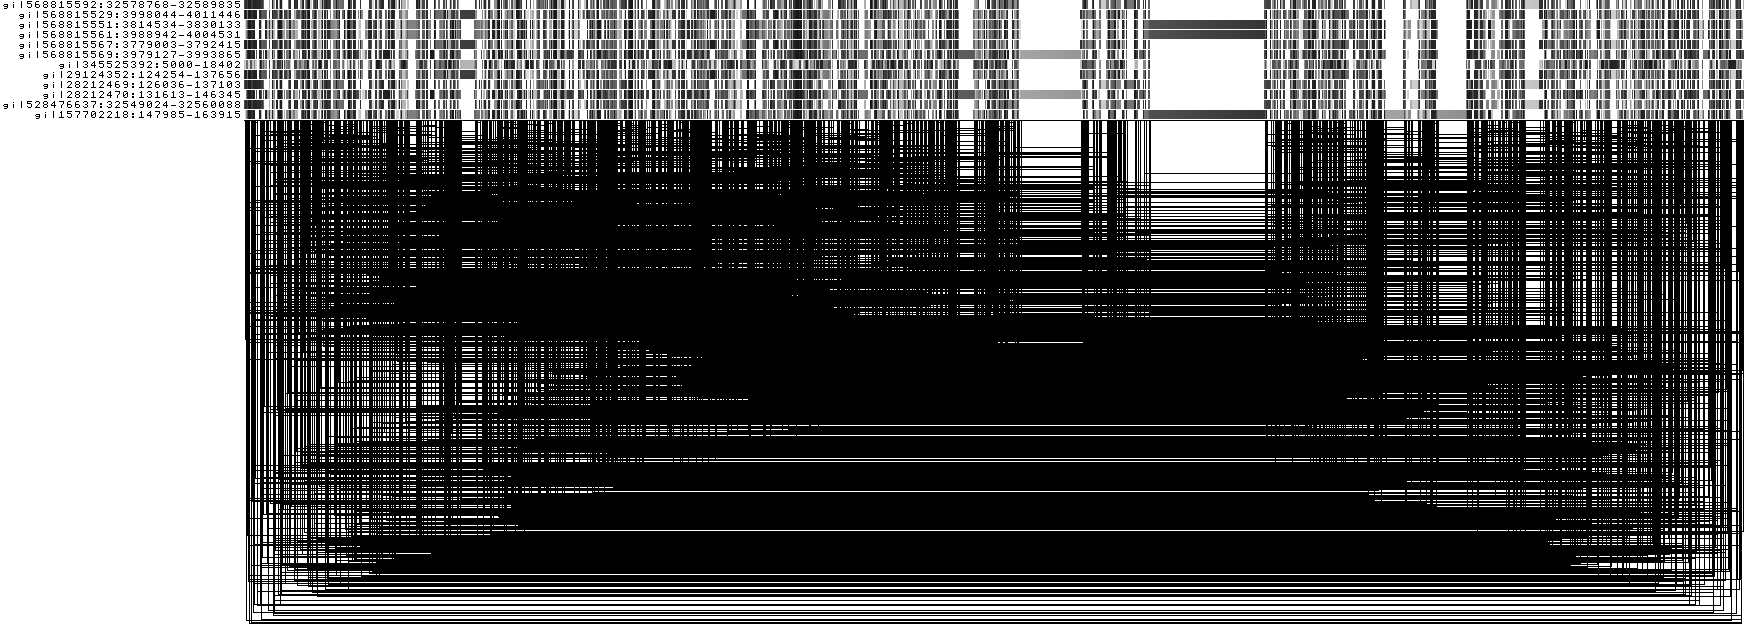
\includegraphics[width=\linewidth]{fig/latent_graph_structure/DRB1-3123.fa.gz.c666522.417fcdf.seqwish.og.r.og.ud.png}
		\label{fig:random_pos}
	\end{subfigure}
	%\smallskip
	\begin{subfigure}[t]{0.4\textwidth}
		\centering
		\caption{}
		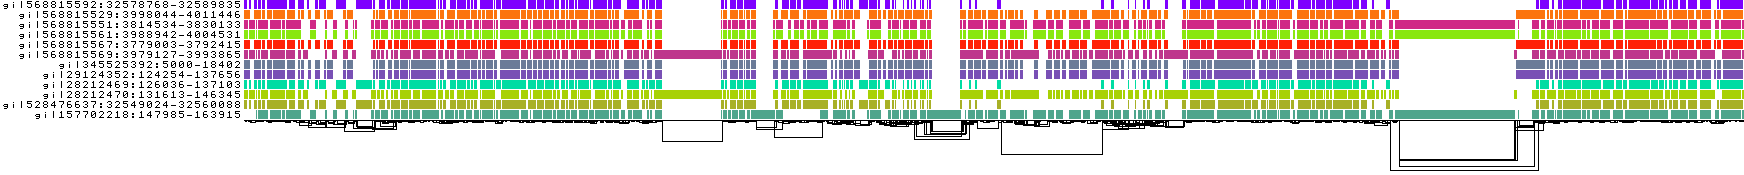
\includegraphics[width=\linewidth]{fig/latent_graph_structure/DRB1-3123.fa.gz.c666522.417fcdf.seqwish.og.Y.og.png}
		\label{fig:sorted}
	\end{subfigure}
	\begin{subfigure}[t]{0.4\textwidth}
		\centering
		\caption{}
		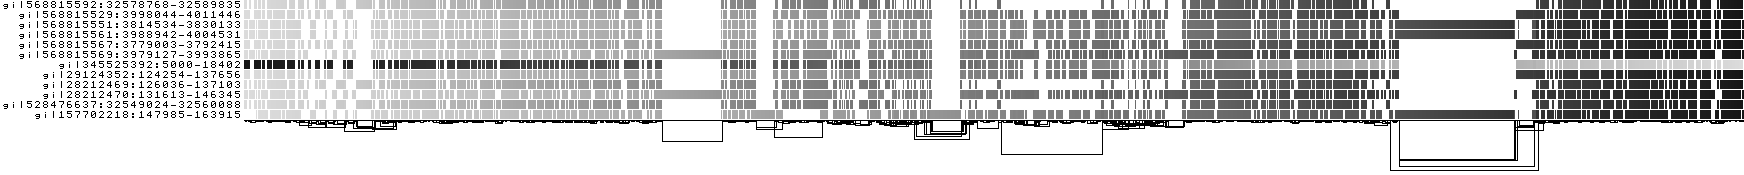
\includegraphics[width=\linewidth]{fig/latent_graph_structure/DRB1-3123.fa.gz.c666522.417fcdf.seqwish.og.Y.og.ud.png}
		\label{fig:sorted_pos}
	\end{subfigure}
	\begin{subfigure}[t]{0.4\textwidth}
		\centering
		\caption{}
		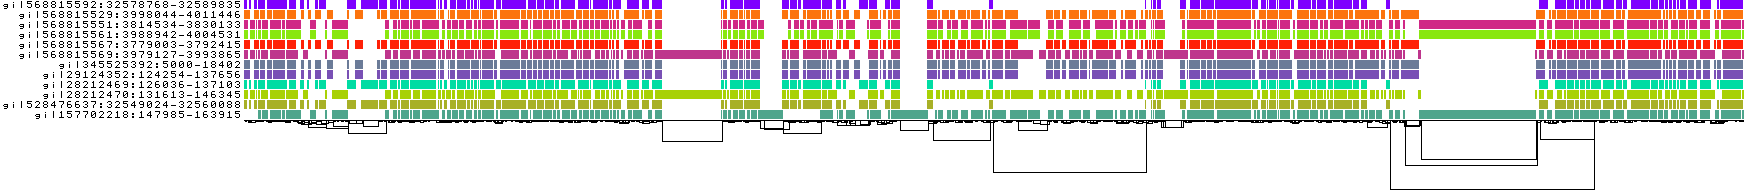
\includegraphics[width=\linewidth]{fig/latent_graph_structure/DRB1-3123.fa.gz.c666522.417fcdf.seqwish.og.Ygs.og.png}
		\label{fig:pipeline}
	\end{subfigure}
	\begin{subfigure}[t]{0.4\textwidth}
		\centering
		\caption{}
		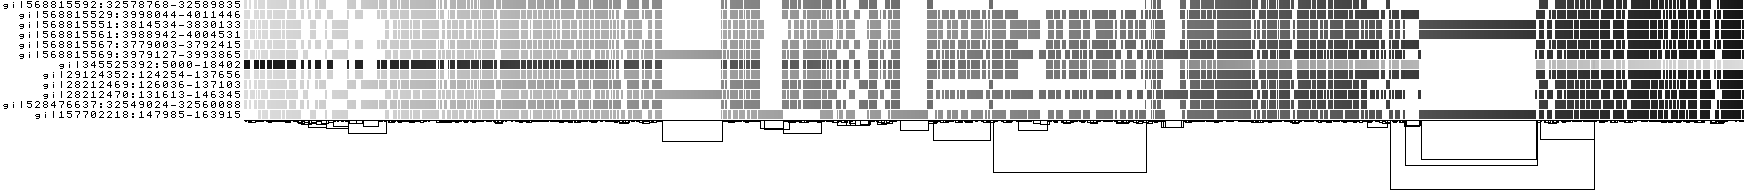
\includegraphics[width=\linewidth]{fig/latent_graph_structure/DRB1-3123.fa.gz.c666522.417fcdf.seqwish.og.Ygs.og.ud.png}
		\label{fig:pipeline_pos}
	\end{subfigure}
	\begin{subfigure}[t]{0.4\textwidth}
		\centering
		\caption{}
		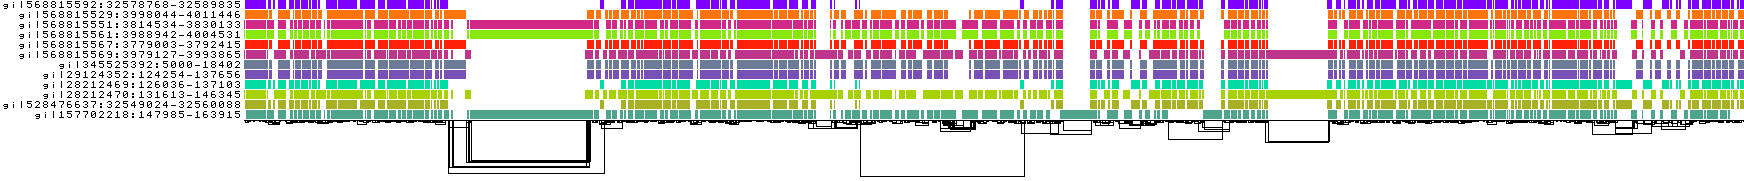
\includegraphics[width=\linewidth]{fig/latent_graph_structure/DRB1-3123.fa.gz.c666522.417fcdf.seqwish.og.YH.og.png}
		\label{fig:ref}
	\end{subfigure}
	\begin{subfigure}[t]{0.4\textwidth}
		\centering
		\caption{}
		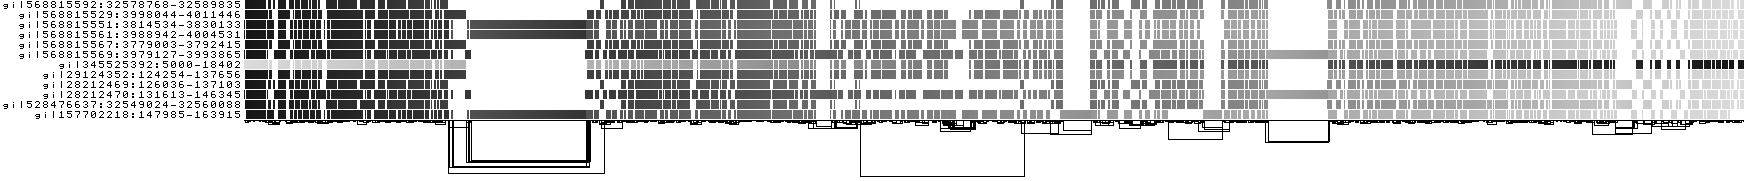
\includegraphics[width=\linewidth]{fig/latent_graph_structure/DRB1-3123.fa.gz.c666522.417fcdf.seqwish.og.YH.og.ud.png}
		\label{fig:ref_pos}
	\end{subfigure}
		\begin{subfigure}[t]{0.8\textwidth}
		\centering
		\caption{}
		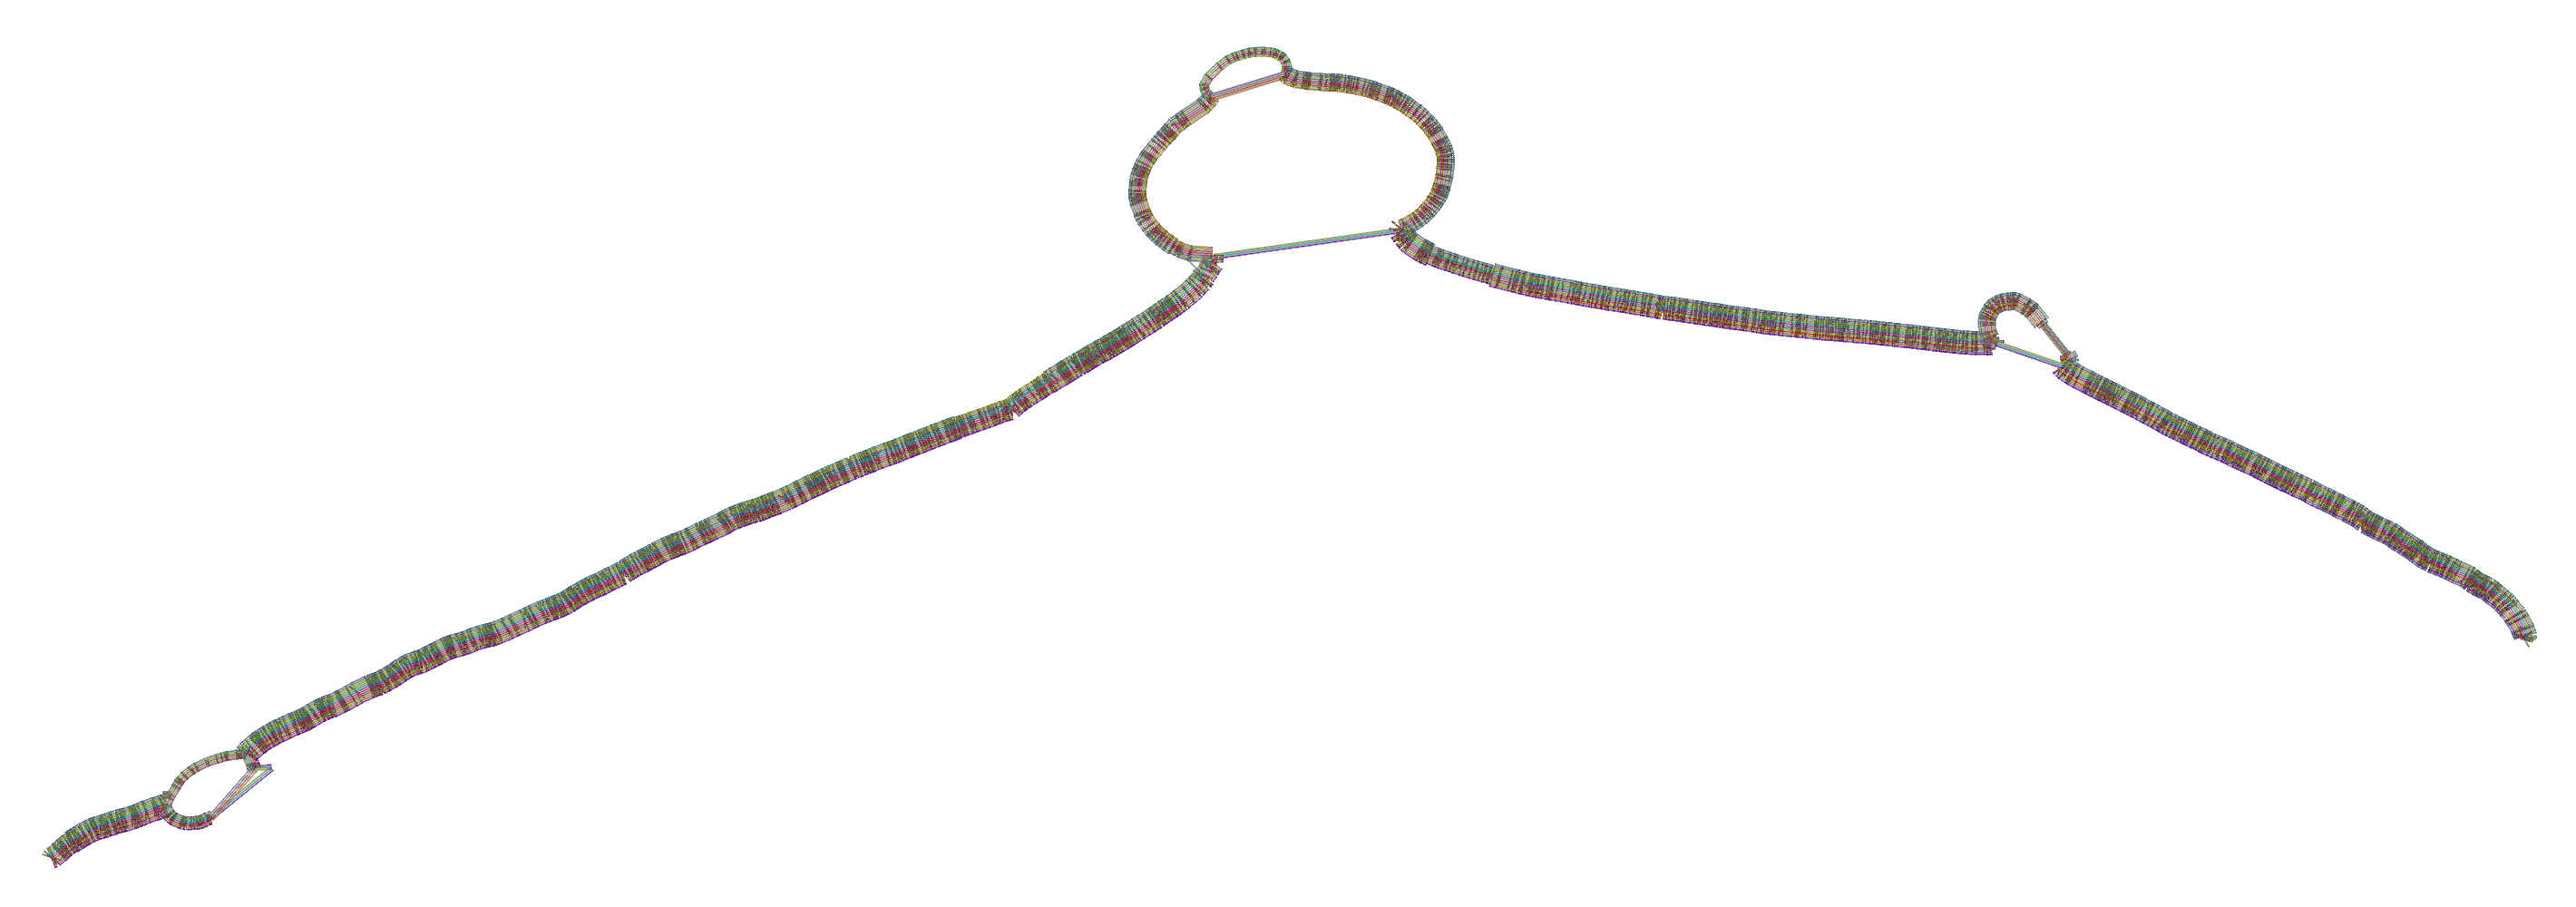
\includegraphics[width=\linewidth]{fig/latent_graph_structure/TODO_2d.png}
		\label{fig:2d}
	\end{subfigure}
	\caption{
		Latent graph structures.
		\textbf{(a)} Randomly sorted graph. \textbf{(b)} Randomly sorted graph by position. \textbf{(c)} PG-SGD sorted graph. \textbf{(d)} PG-SGD sorted graph by position. \textbf{(e)} Ygs sorted graph. \textbf{(f)} Ygs sorted graph by position. \textbf{(g)} Reference sorted graph. \textbf{(h)} Reference sorted graph by position. \textbf{(i)} 2D layout of graph.
	}
	\label{fig:latent_graph_structure}
\end{figure*}
Table 2: Metrics of the sorted graphs in Fig. 3.
\begin{table}[]
	\caption{Metrics of the latent graphs.}
	\begin{tabular}{|l|l|l|l|l|}
		\hline
		& RANDOM & Y & Ygs & Ref \\ \hline
		METRIC 1 &        &   &     &     \\ \hline
		METRIC 2 &        &   &     &     \\ \hline
	\end{tabular}
\end{table}
\paragraph{Bonus Section}
Fig. 4: Detect tension. Relax a graph. Detect tension afterwards.
I need to test this on a new data set I got from Erik.
I need to establish a fixed lower boundary for the tension from which on we don't relax anymore. \\
With a high quality layout, we can measure the discrepancy of the path layout position versus the expected path nucleotide position, the “tension” of a graph.
The greater the “tension”, the greater is the possibility of a biologically meaningless alignment.
This allows us to detect telomere collapsing alignment errors and hopefully (pangenome) assembly errors, subsequently correcting them.
\begin{figure*}[!htb]
	\centering
	%\hline
	\begin{subfigure}[t]{0.4\textwidth}
		\centering
		\caption{}
		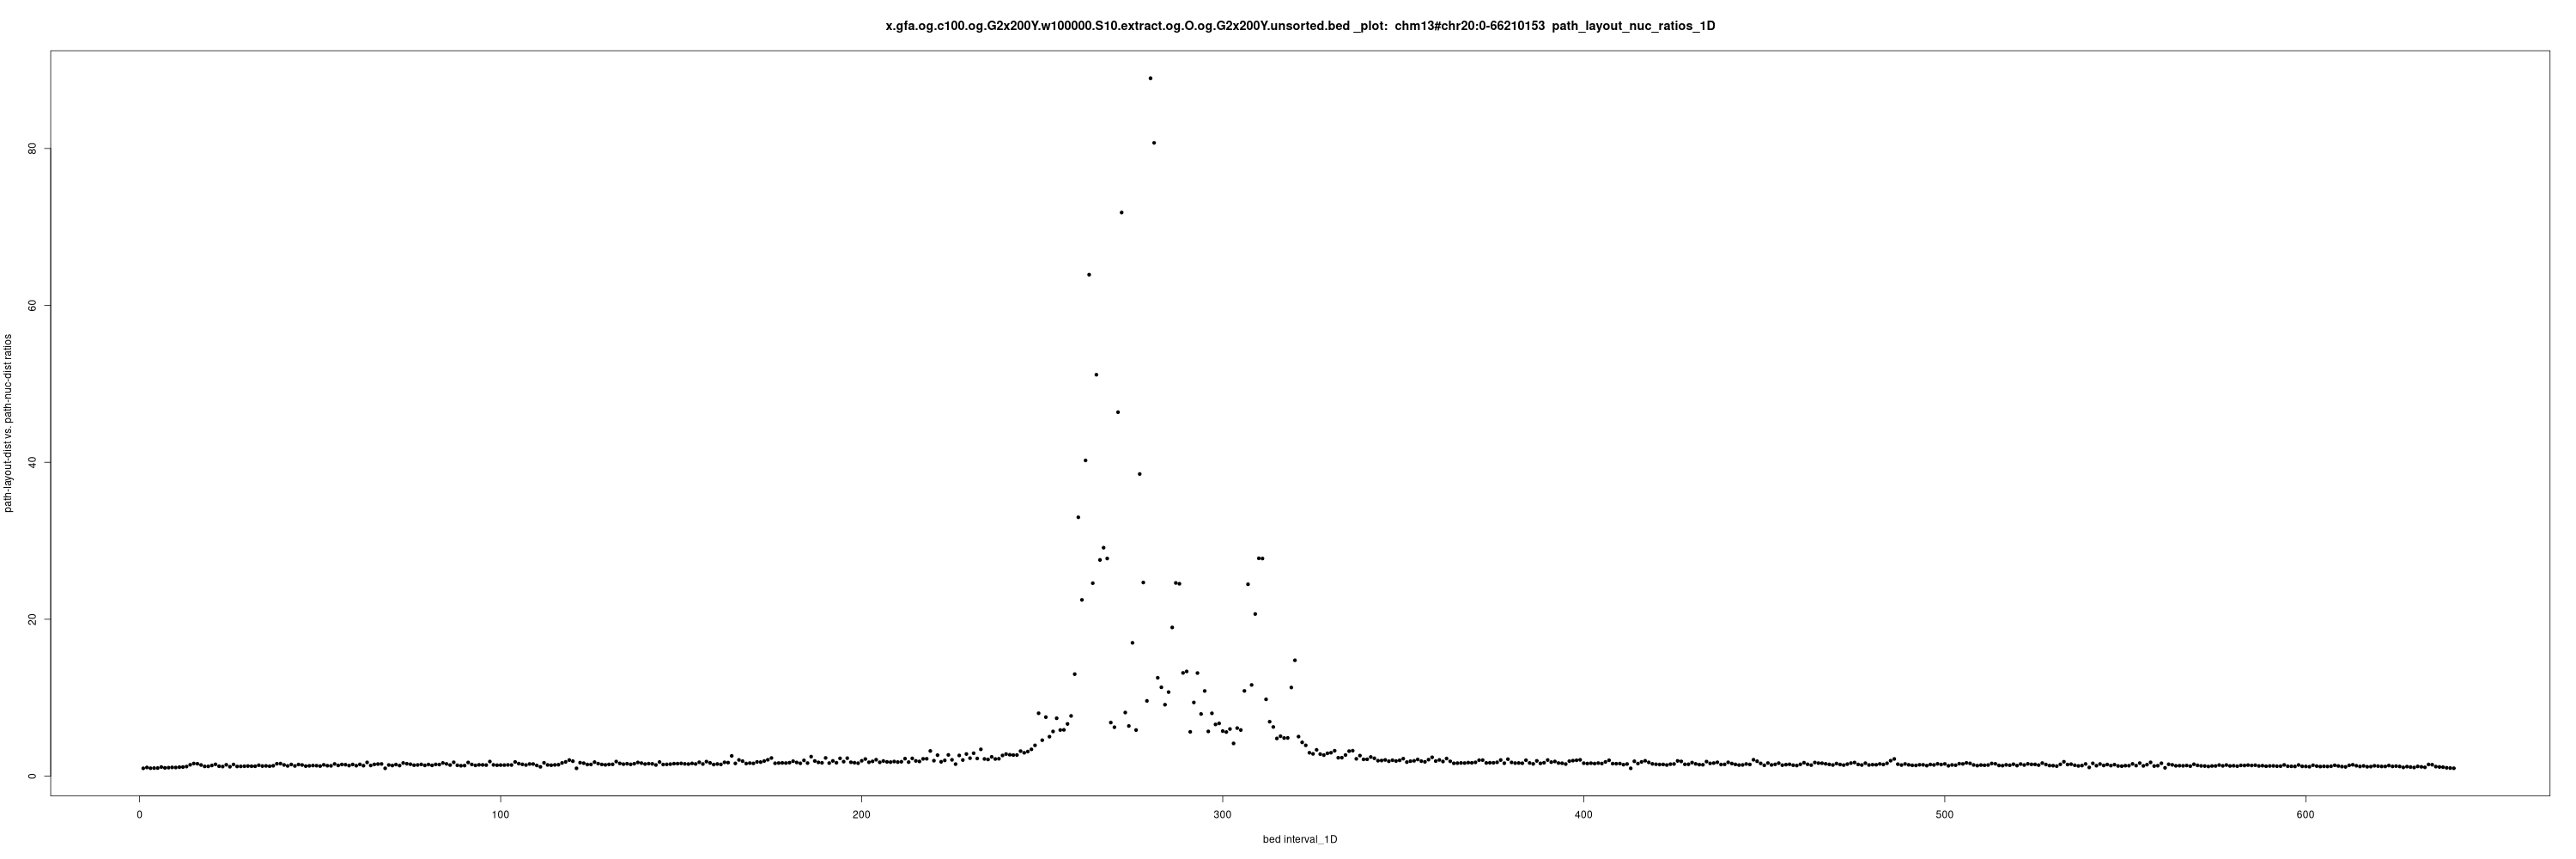
\includegraphics[width=\linewidth]{fig/tension/tension_bed.png}
		\label{fig:tension_bed}
	\end{subfigure}
	\begin{subfigure}[t]{0.4\textwidth}
		\centering
		\caption{}
		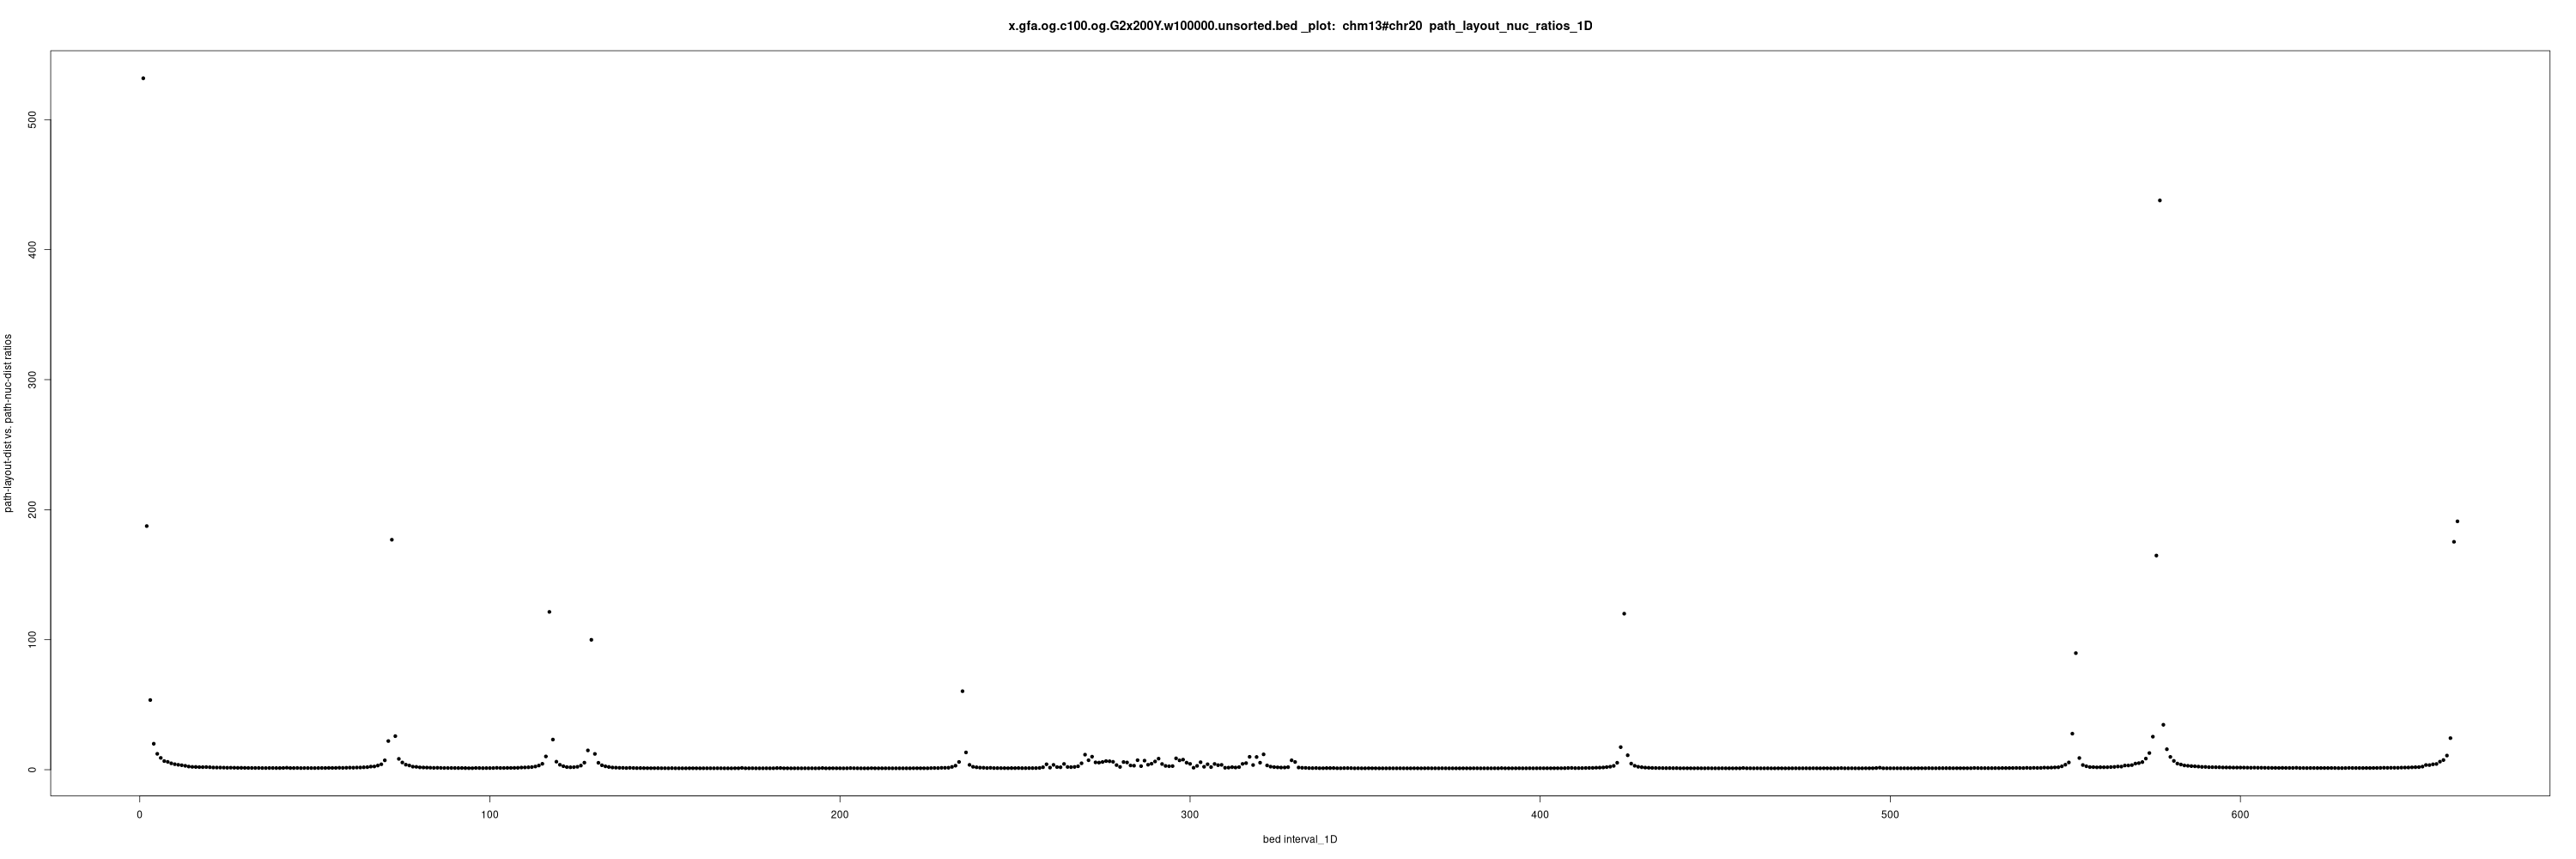
\includegraphics[width=\linewidth]{fig/tension/tension_bed_relaxed.png}
		\label{fig:tension_extracted}
	\end{subfigure}
\\
	%\smallskip
	\begin{subfigure}[t]{0.1\textwidth}
		\centering
		\caption{}
		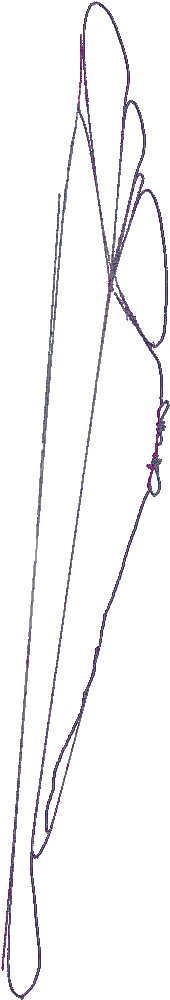
\includegraphics[width=\linewidth]{fig/tension/layout.png}
		\label{fig:tension_draw}
	\end{subfigure}
	\begin{subfigure}[t]{0.1\textwidth}
		\centering
		\caption{}
		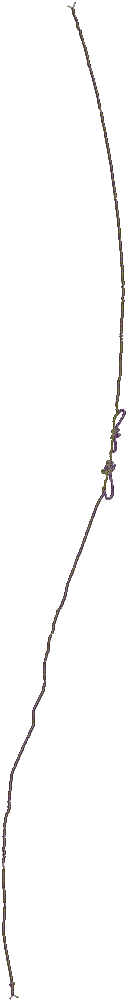
\includegraphics[width=\linewidth]{fig/tension/layout_relaxed.png}
		\label{fig:tension_draw_extracted}
	\end{subfigure}
	\caption{
		Detecting tension and relaxing a pangenome graph.
		\textbf{(a)} Tension detection before relaxation. \textbf{(b)} Tension detection after relaxation. \textbf{(c)} Folded 2D before relaxation. \textbf{(d)} Linearized 2D after relaxation.
	}
	\label{fig:tension}
\end{figure*}

\section{Discussion}
\label{sec:discussion}

We propose / implemented ....
\paragraph{}
Difference to other existing methods, are there possible improvements of our method possible?
\paragraph{}
Discuss performance eval
@Jiajie + Niklas: What about going GPU?
\paragraph{}
The algorithm allows to inspect a pangenome graph on base-level, as a whole.
\paragraph{from the ODGI paper:}
Its static, large-scale 1D and 2D visualizations of the pangenome graphs allow an unprecedented high-level perspective on variation in pangenomes, and have also been critical in the development of pangenome graph building methods.
However, an interactive solution that combines the 1D and 2D layout of a graph with annotation and read mapping information across different zoom levels is still missing.
Recent interactive pangenome graph browsers are reference-centric (Beyer et al., 2019; Yokoyama et al., 2019), have a limited predefined coordinate system (Durant et al., 2021), or focus primarily on 2D representations (Gonnella et al., 2019; Wick et al., 2015).
Our graph sorting and layout algorithms can provide the foundation for future tools of this type.
We plan to focus on using these learned models to detect structural variation and assembly errors.
\paragraph{}
The graph simplification pipeline smoothxg runs POA for each block of paths that are co-linear within each seqwish induced variation graph.
A prerequisite is that the graph nodes are sorted according to their occurrence in the graph's embedded paths.
Our 1D path-guided SGD algorithm is designed to provide this kind of sort.
Already, the 1D PG-SGD is a key step in the PanGenome Graph Building (PGGB) pipeline that we successfully applied to build the first draft human pangenome reference (Liao et al., bioRxiv 2022).
\paragraph{}
I'd like to argue that this projection presents biologically relevant structures that we can work with downstream
both for human interface
and for other algorithms that look at and classify variation
\paragraph{}
What about the future?
\paragraph{}
How can other scientists benefit from this work?
Graph visualization (together with annotation) is key for understanding variations.
This projection presents biologically relevant structures that we can work with downstream for researches and algorithms that look at and classify variation,

\section*{Acknowledgments}

We are grateful to members of the HGSVC and HPRC production teams for their development of resources used in our exposition.
We thank the authors of the pangenome resources made available on GenBank which have made our experiments possible.

\section*{Funding}

JNM.S., J.L., and Z.Z. acknowledge funding from the NSF PPoSS Award \#2118709.
S.H. acknowledges funding from the Central Innovation Programme (ZIM) for SMEs of the Federal Ministry for Economic Affairs and Energy of Germany.
S.N. acknowledges Germany’s Excellence Strategy (CMFI), EXC-2124 and (iFIT)—EXC 2180–390900677.
This work was supported by the BMBF-funded de.NBI Cloud within the German Network for Bioinformatics Infrastructure (de.NBI) (031A532B, 031A533A, 031A533B, 031A534A, 031A535A, 031A537A, 031A537B, 031A537C, 031A537D and 031A538A).
A.G. acknowledges efforts by Nicole Soranzo to establish a pangenome research unit at the Human Technopole in Milan, Italy.

\section*{Competing interests}
The authors declare that they have no competing interests.

\section*{Data availability}

Code and links to data resources used to build this manuscript and its figures can be found in the paper's public repository: \url{https://github.com/pangenome/sorting-paper}.

\bibliographystyle{natbib}

\bibliography{document}

\end{document}
